\section{One big experiment}\label{sec:1}
Let $P = \num{10000}$ and $X = 1$. Since only one experiment is done,
\cref{eq:pi_final} cannot be used to calculate the uncertainty. Because of that
the uncertainty is defined as
\begin{equation}
	\Delta \pi_x = \sqrt{\text{Var}(4[X^2 + Y^2 \leq 1])}
    \label{eq:uncertainty_for_one_x}
\end{equation}
with $\text{Var}(X)$ being the variance of the random variable $X$.
Letting the experiment run results in a value of
\begin{equation}
	\pi_x = \num{3.1 \pm 1.7},
\end{equation}
which is considering the uncertainty of approximately \per{53} close to the real value.\par
%
When doing just one experiment, the distribution of the generated points is 
of interest. For this the histogram of the radii $R = \sqrt{X^2 + Y^2}$
and the squared radii are plotted in \cref{fig:radii_hist,fig:radii_squared_hist}.
For the radii we can see a linear rising distribution with a maximum at $r=1$, after which 
the distribution drops. This drop is also visible for the squared radii, but 
in the region $[0,1]$ a constant distribution is visible. The drop after 
$r=1$ is easily explainable with the fact that points insied a $2\times 2$ square
we generated and a circle with radius $1$ is the biggest circle that fits inside.
Whith this in mind the amount of points generated on the circumference of a 
circle with bigger radius has to get smaller.
\textbf{TO BE CONTINUED}


\begin{figure}[h!]
    \centering
    \begin{minipage}{.45\linewidth}
        \centering
        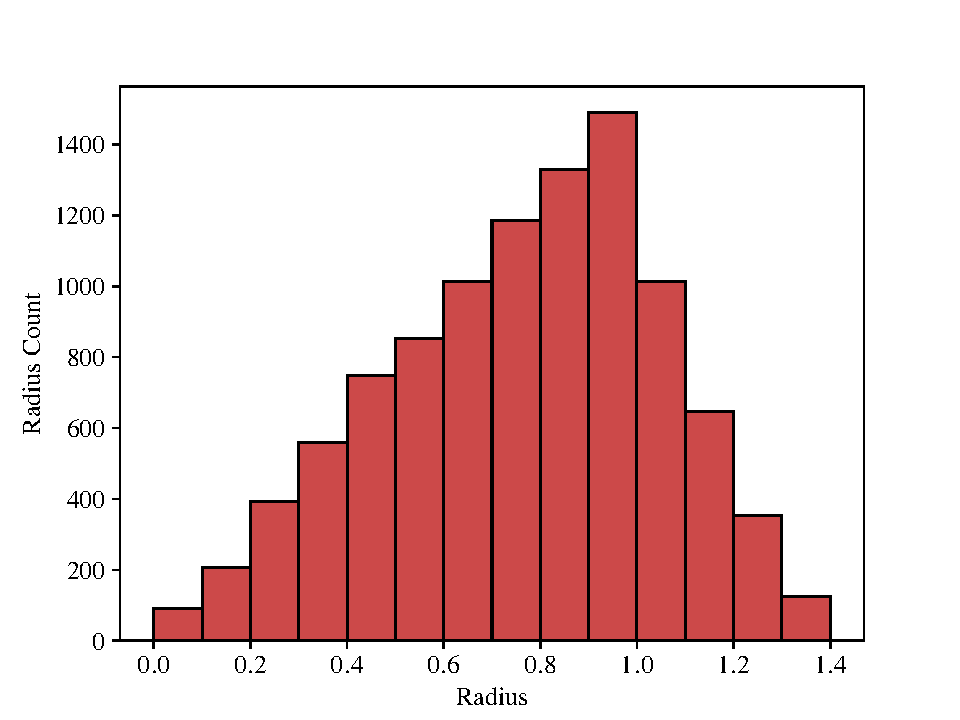
\includegraphics[width=\linewidth]{figs/ex1.1_radii_hist.pdf}
        \caption{Histogram of radii from all the generated points of one big experiment
            with $P=\num{10000}$.}
        \label{fig:radii_hist}
    \end{minipage}
    \hfill
    \begin{minipage}{.45\linewidth}
        \centering
        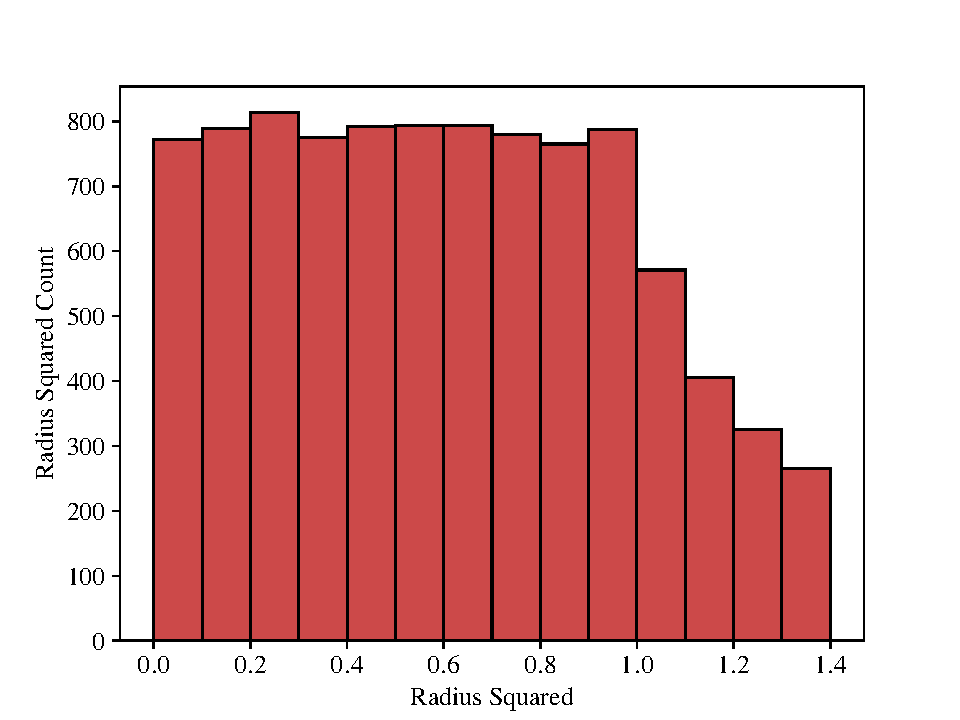
\includegraphics[width=\linewidth]{figs/ex1.1_radii_squared_hist.pdf}
        \caption{Histogram of the squared radii from all the generated points of one big experiment
            with $P=\num{10000}$.}
        \label{fig:radii_squared_hist}
    \end{minipage}

\end{figure}

\begin{figure}[h]
    \centering
    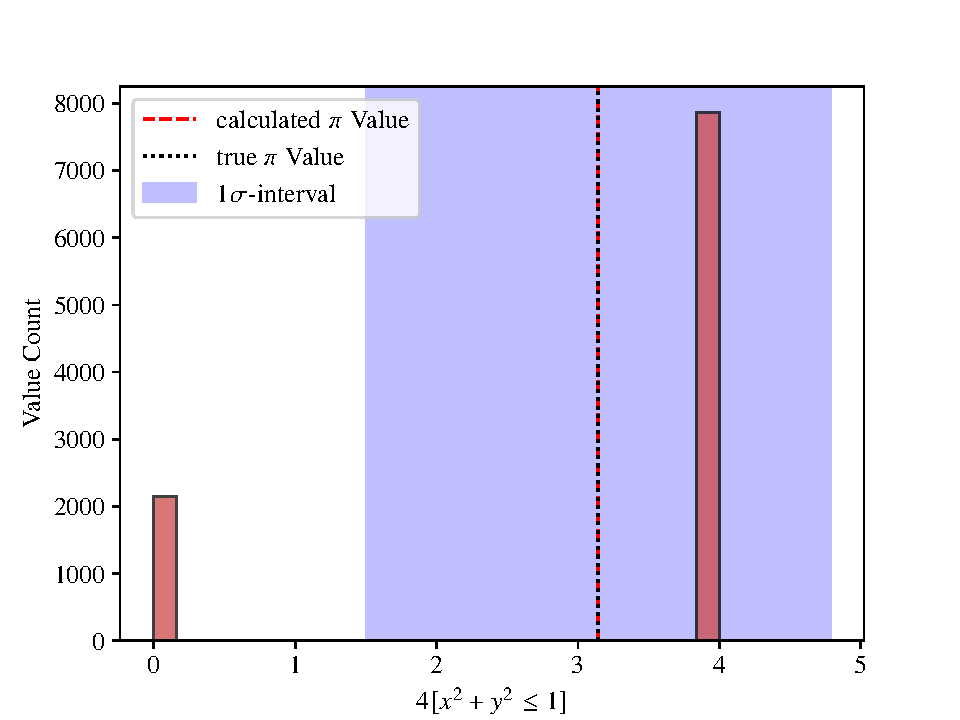
\includegraphics[width=.6\linewidth]{figs/ex1.1_indicator_hist.pdf}
    \caption{Histogram of the indicator variable $[X^2 + Y^2 \leq 1]$ for an experiment 
        with $P = \num{10000}$.}
\end{figure}